\subsection{Usage Behavior}
\label{subsec:behavior}

We aggregate the the usage behavior of households both over space (i.e., distinct devices)
and over time (i.e., over each day in the same time slot). We observe that the variance in
daily network usage during weekdays is much higher as compared to weeknights and holidays.
Thus, we divide our analysis based on day of the week in figure~\ref{fig:TS-data-rate-daily}. 

We find that the daily usage behavior on the weekend and holiday usage has four parts:
(a) an initial sharp rise, (b) a flatter rise, (c) sharp rise to evening, (d) sharp decrease
after 12 am. In contrast, weekdays clearly have two parts in a normal working day: (a) a rise
in data usage from 7:00 AM that peaks in late evening around 8:00 PM, and (b) a sharp fall in
usage from 12:00 PM to 6:00 AM in the morning. This pattern does not show any trough in the
median network usage. This is in contrast to the aggregated usage patterns observed at ISPs
that show a local small peak in network load in the morning (10AM), then dip in the afternoon,
and then rise up again in the late evening hours. ~\cite{sandvine2014report1},
\todo{confirm sandvine, check dasu shows this, check other studies.}

\begin{figure}[ht!]
\begin{minipage}{\linewidth}
  \centering
  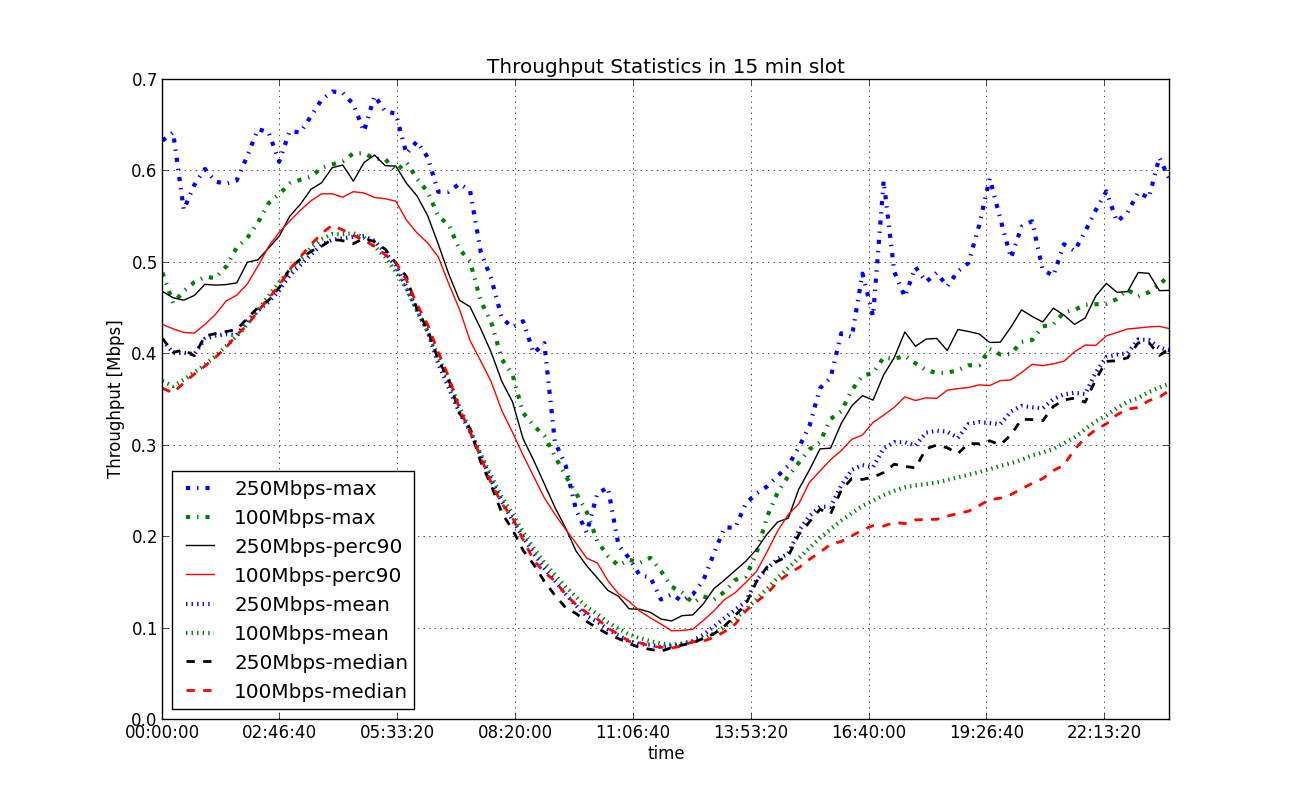
\includegraphics[width=\linewidth]{figures/describe-total-throughput-per-day[replace].png}
  \caption{agg (days) over means (devices): aggregate has no trough, peaks in the evening hours}
  %http://riverside.noise.gatech.edu:8083/separated/full/describe-total-throughput-per-day.png
  \label{fig:TS-data-rate-daily}
\end{minipage}
\end{figure}

Figure ~\ref{fig:TS-data-rate-daily} alse shows that the peak hour behavior of both sets
is very similar, but during the day, the median data rate of \test set devices is slightly
higher \todo{quantify} than the \control set. 

\todo{make two sub plots for (a) test and (b) control: (mean of day) (sum of device) bytes,
include (perc90 of day) (sum of device) bytes and (median of day) (sum of device) bytes.
Purpose is to show patterns individually, not compare differences. Patterns to show are (1)
no troughs in usage, (2) prime-time hours shift (subsection ~\ref{subsec:primetime}), (3)
difference between 90\%-ile and median (subsection ~\ref{subsec:peakratio})}

\todo{separate subplots for M-F and S/S/holidays -- choose two interesting ones}

\todo{Also, test set seems to have this small peak and a trough, but control doesn't. Why??. Test and control medians differ during office hours (10:00 AM to 6:00 PM) but are similar in peak hours...}
%see: http://sites.noise.gatech.edu/~sarthak/files/comcast/plots/full_dw/describe-total-throughput-per-day-ALL.png

%This lack of troughs could be the result of the users' behavior in higher tier
%bandwidth, and motivated us  to further study user taxonomy in
%section~\ref{subsec:peakratio}.